\documentclass{scrreprt}
\usepackage{listings}
\usepackage{array}
\usepackage{longtable}
\usepackage{tikz} 
\usepackage{underscore}
\usepackage[x11names]{xcolor} 
\usepackage{array} 
\setlength{\arrayrulewidth}{0.5mm} 
\setlength{\tabcolsep}{12pt} 
\renewcommand{\arraystretch}{1.5} 
\usepackage[bookmarks=true]{hyperref}
\usepackage[utf8]{inputenc}
\usepackage[table,xcdraw]{xcolor}
\usepackage[english]{babel}
\usepackage{enumitem}
\usepackage{longtable}
\usepackage[a4paper, margin=1in]{geometry}
\usetikzlibrary{shapes, arrows.meta, positioning, backgrounds}
\usetikzlibrary{arrows.meta}
\usetikzlibrary{shapes.geometric, positioning, arrows.meta}
\usetikzlibrary{shapes.geometric, positioning, arrows.meta}
\usetikzlibrary{positioning}
% Define styles for different node types
\tikzstyle{startstop} = [rectangle, rounded corners, minimum width=3cm, minimum height=1cm, text centered, draw=black, fill=red!30]
\tikzstyle{process} = [rectangle, minimum width=3.5cm, minimum height=1cm, text centered, draw=black, fill=blue!30]
\tikzstyle{arrow} = [thick,->,>=stealth]
% Define stickman style
\tikzset{
    startstop/.style={
        rectangle, rounded corners, minimum width=3cm, minimum height=1cm, text centered, draw=black, fill=gray!30
    },
    process/.style={
        rectangle, minimum width=3cm, minimum height=1cm, text centered, draw=black, fill=blue!30
    },
    decision/.style={
        diamond, aspect=2, minimum width=3cm, minimum height=1cm, text centered, draw=black, fill=orange!30
    },
    arrow/.style={
        thick, ->, >=stealth
    },
    stickman/.pic={
        % Head
        \draw[fill=gray] (0,0.6) circle (0.3cm);
        % Body
        \draw[line width=0.5mm] (0,0.3) -- (0,-0.6);
        % Arms
        \draw[line width=0.5mm] (-0.4,0.3) -- (0.4,0.3);
        % Legs
        \draw[line width=0.5mm] (0,-0.6) -- (-0.4,-1.2);
        \draw[line width=0.5mm] (0,-0.6) -- (0.4,-1.2);
}
}

\hypersetup{
    bookmarks=false,    % show bookmarks bar?
    pdftitle={Software Requirement Specification},    % title
    pdfauthor={Jean-Philippe Eisenbarth},                     % author
    pdfsubject={TeX and LaTeX},                        % subject of the document
    pdfkeywords={TeX, LaTeX, graphics, images}, % list of keywords
    colorlinks=true,       % false: boxed links; true: colored links
    linkcolor=blue,       % color of internal links
    citecolor=black,       % color of links to bibliography
    filecolor=black,        % color of file links
    urlcolor=purple,        % color of external links
    linktoc=page            % only page is linked
}
\usetikzlibrary{shapes, arrows.meta, positioning, backgrounds}

\tikzstyle{startstop} = [rectangle, rounded corners, minimum width=3cm, minimum height=1cm, text centered, draw=black, fill=red!30]
\tikzstyle{process} = [rectangle, minimum width=3.5cm, minimum height=1cm, text centered, draw=black, fill=blue!10]
\tikzstyle{database} = [rectangle, minimum width=3cm, minimum height=1cm, text centered, draw=black, fill=orange!30]
\tikzstyle{auth} = [rectangle, minimum width=3cm, minimum height=1cm, text centered, draw=black, fill=green!30]
\tikzstyle{ui} = [rectangle, minimum width=3.5cm, minimum height=1cm, text centered, draw=black, fill=yellow!30]
\tikzstyle{arrow} = [thick,->,>=stealth]


\usepackage{hyperref}
\begin{document}

\begin{titlepage}
    \centering
    \begin{center}
        
\includegraphics[width=0.5\textwidth]{./logo.png} % Adjust width as necessary
    \end{center}
\begin{center}
    \textbf{Department of Computer Science and Engineering}\\
    Premier University
\end{center}
\begin{center}
    \textnormal{ CSE306: Software Engineering \& Information System Design Laboratory }
\end{center}
    \huge
    \textbf{Final Report}\\
    \vspace{0.5in}
    \LARGE
    \textbf{Odyssey Travel Agency Software}\\
    \vspace{1in}
    \large
    \textbf {Submitted by}\\
    \begin{center}
        \renewcommand{\arraystretch}{1.5} % Adjusts vertical spacing in the table
        \begin{tabular}{|>{\raggedright\arraybackslash}p{0.6\textwidth}|p{0.3\textwidth}|} % Adjust column widths
        \hline
        \textbf{Name} & \textbf{ID} \\
        \hline
        Mohammad Hafizur Rahman Sakib & 0222210005101118 \\
        \hline
        Arnab Shikder & 0222210005101098 \\
        \hline
        Mohammad Ohidul Alam & 0222210005101123 \\
        \hline
        Sayed Hossain & 0222210005101102 \\
        \hline
        Mohammad Asmual Hoque Yousha & 0222210005101121 \\
        \hline
        \end{tabular}
        \end{center}
    \vspace{0.5in}
 
\begin{minipage}[t]{0.5\textwidth}
        \textbf{Submitted to :}
        \\Jannatul Maowa Hasi
        \\Lecturer,Department of CSE
        \\ Premier University
        \\ Chittagong
    \end{minipage}%
    \begin{minipage}[t]{0.6\textwidth}
        \raggedleft
        \textbf{Remarks}\\
        \vspace{0.5cm} % Adjust vertical space for remarks
        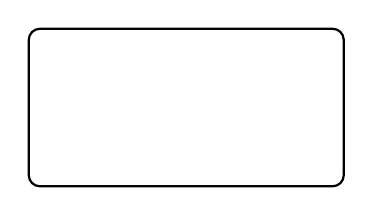
\begin{tikzpicture}
            \draw[thick, rounded corners] (0,0) rectangle (4,2);
        \end{tikzpicture}
    \end{minipage}

    \date{\today}
    \vfill
\end{titlepage}
\newpage



\tableofcontents
\begin{center}   
\end{center}

\chapter{Introduction}
The purpose of this document is to provide a comprehensive description of the webbased project named ”Odyssey Travels,” developed using Next.js. It aims to outline the
system’s objectives, functionalities, user interfaces, operational constraints, and how it
handles external interactions. This document serves as a detailed guide for stakeholders
and developers involved in the project, ensuring a clear understanding of the system’s
scope and requirements. It will define how ”Odyssey Travels” enhances the online travel
booking experience through innovative features and responsive web interfaces.
This web-based application, ”Odyssey Travels,” is designed to enhance user efficiency
and streamline travel planning processes. It aims to empower users by providing intuitive tools to manage and prioritize travel itineraries and bookings seamlessly. Users
will no longer need to rely on traditional methods like spreadsheets or multiple websites to organize their travel plans. ”Odyssey Travels” will enable users to categorize
and prioritize travel activities effortlessly, ensuring optimal utilization of their time and
resources. By offering clear insights into itinerary management and suggesting efficient
scheduling of activities, the application enhances user productivity while maintaining
ease of use. Specifically, the system will guide users in making informed decisions about
their travel plans, suggesting ideal times for activities to maximize efficiency throughout
their journey. It will help users save valuable time by centralizing booking processes
and providing real-time updates on travel arrangements. Additionally, the application
will assist users in optimizing their itineraries by recommending adjustments or identifying unnecessary tasks, ensuring that their travel experiences are both productive and
fulfilling. Overall, ”Odyssey Travels” aims to revolutionize the travel planning experience by offering a user-friendly interface that simplifies task management and enhances
productivity, thereby meeting the diverse needs of modern travelers.


\chapter{System Architecture}
The system architecture of the Odyssey Travel website is designed to provide a robust and scalable platform for managing travel bookings and related services. It comprises several key components:

\section{System Architecture Diagram}

{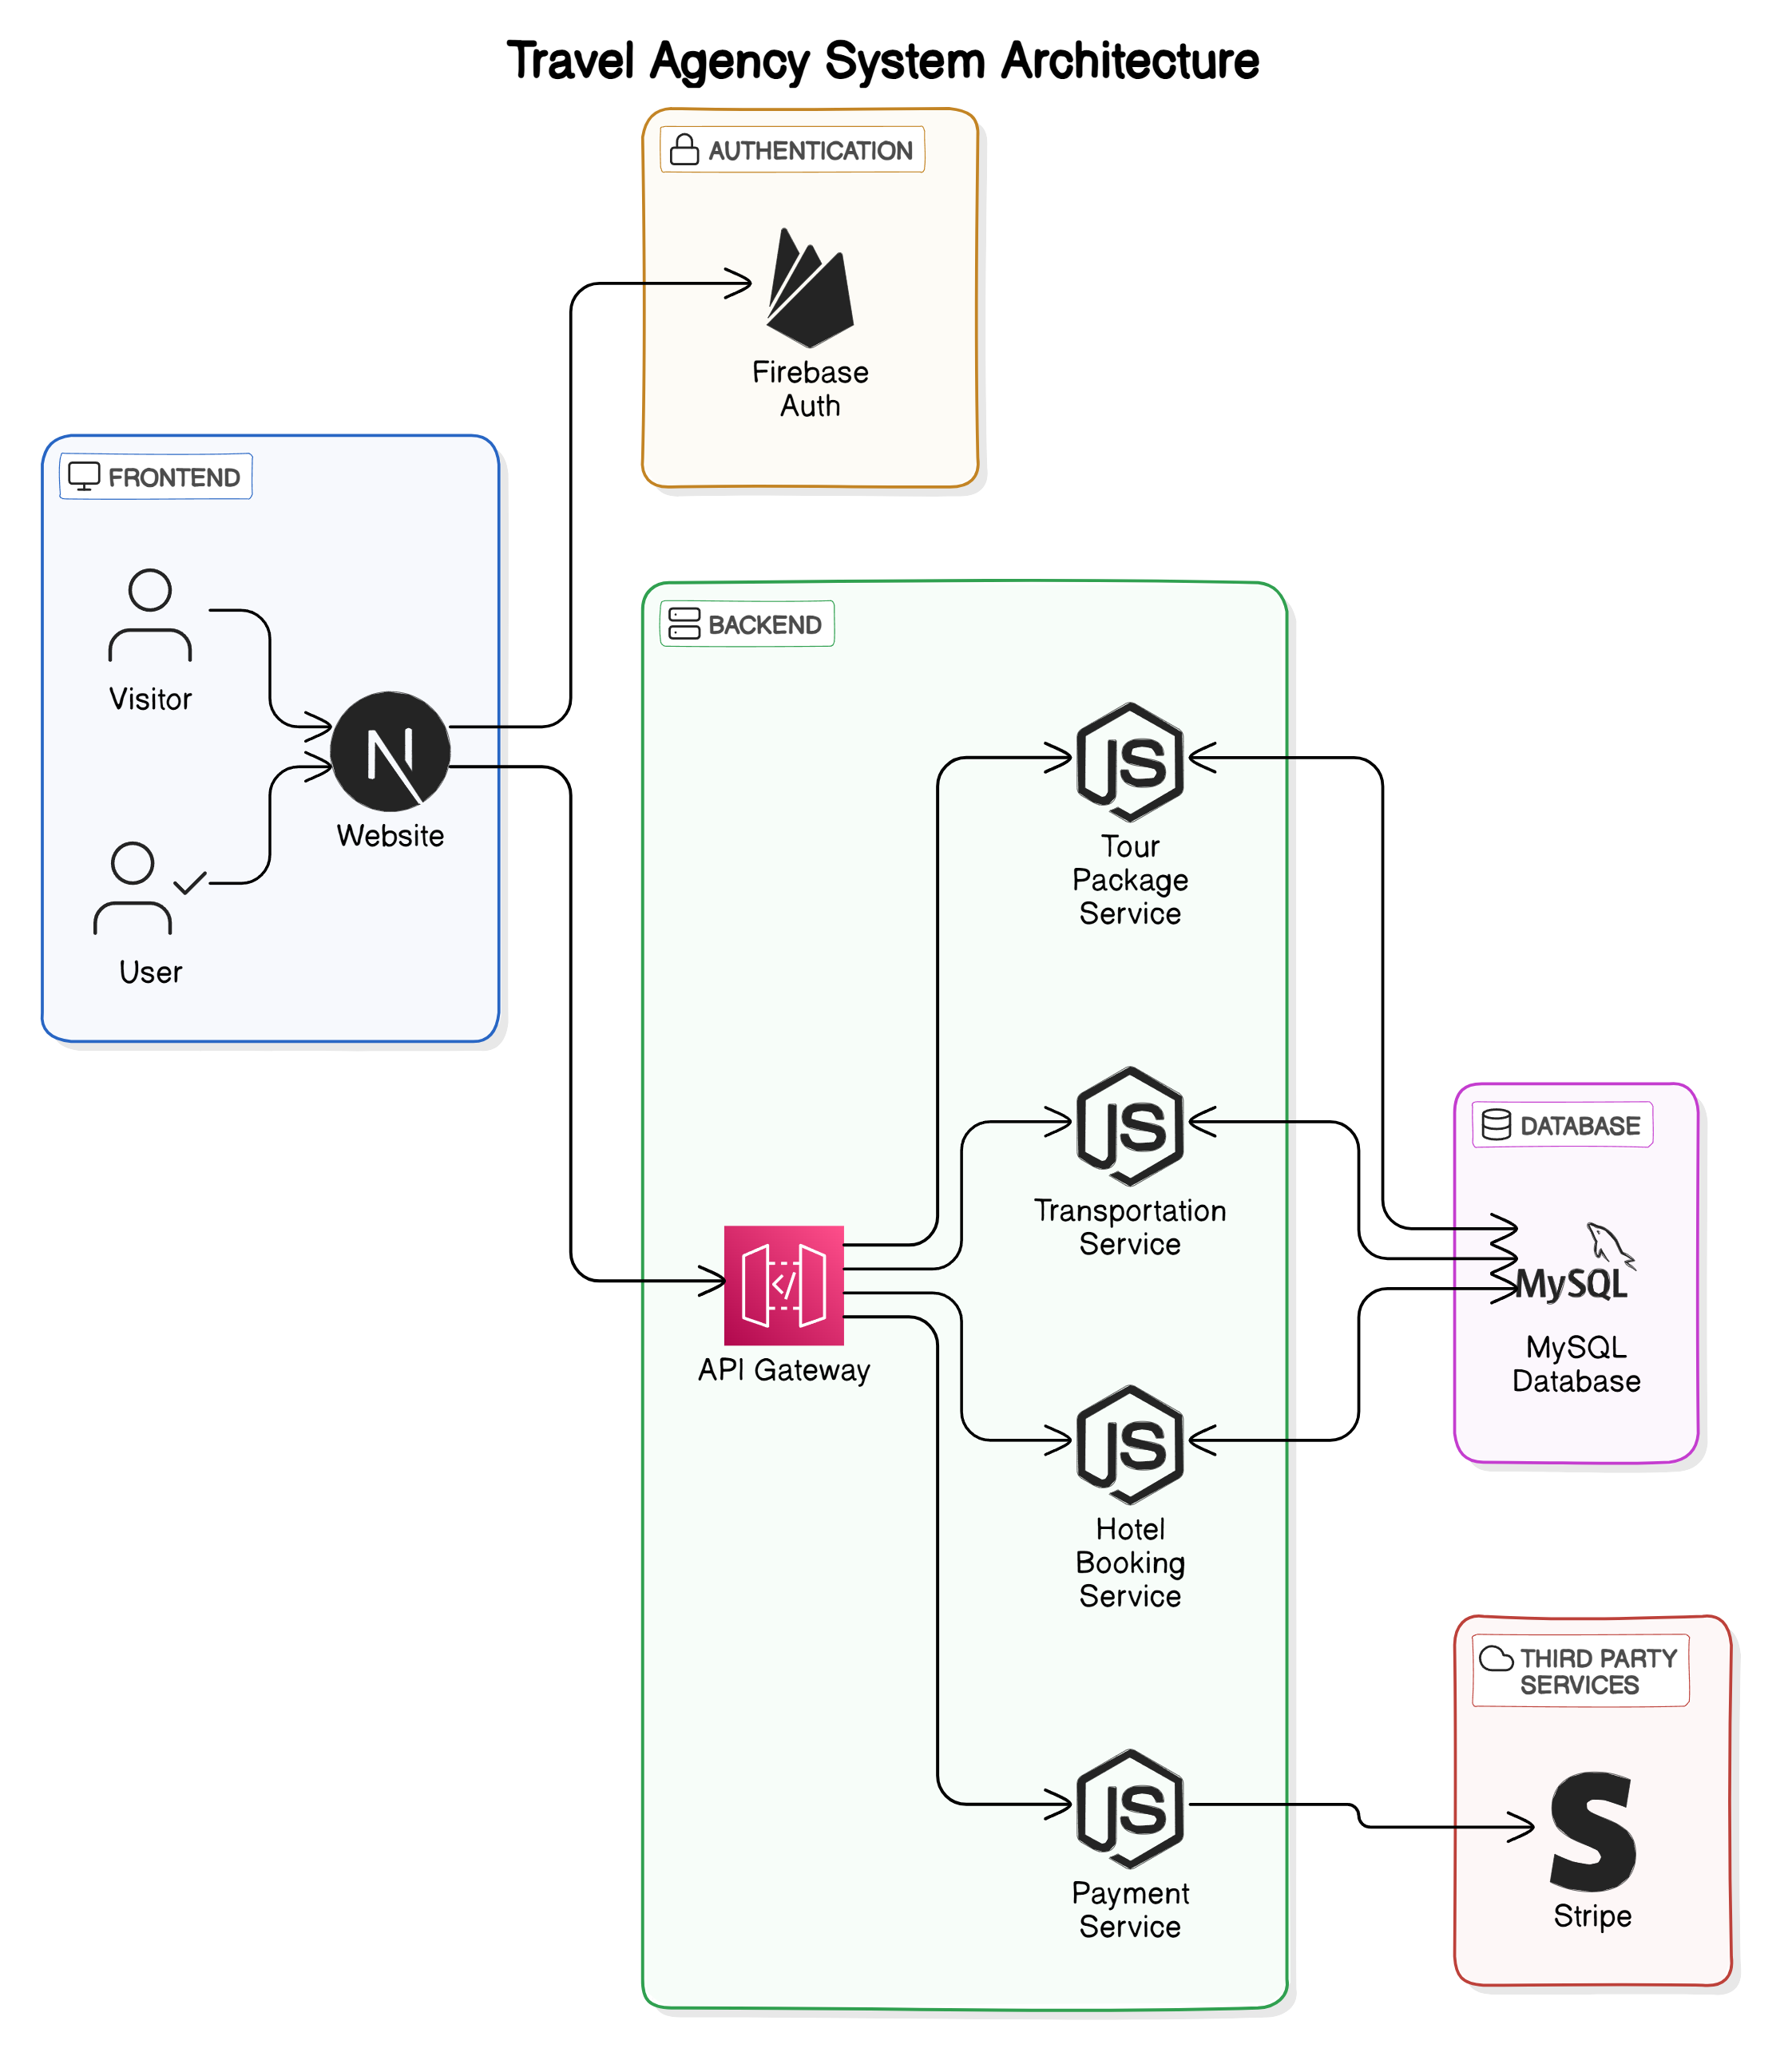
\includegraphics[width=500px, height=480px]{SAD.png}}

\begin{center}
    \parbox{0.8\textwidth}{ 
        \centering
        \textbf{Figure - 2.1 : System Architecture Diagram For Travel Agency Software}
    }
\end{center}

\section{System Architecture Overview}

The system architecture of \textbf{Odyssey Travels} is designed to efficiently manage travel planning and booking processes. It is structured around a web-based software application that interacts with various user types—visitors, registered users, and administrators.

\subsection{Client-Side (Frontend)}
The user interface is built using \textbf{Next.js}, a React framework that supports server-side rendering for fast and efficient page loads. The application is optimized for both desktop and mobile devices, ensuring a responsive and user-friendly experience. Key features include browsing travel packages, booking accommodations, and managing user profiles. The interface components are designed to be intuitive, allowing users to navigate the site easily.

\subsection{Server-Side (Backend)}
The backend handles all data processing and business logic. It uses RESTful APIs to manage communication between the client-side and server-side components. The server processes user requests, interacts with databases to retrieve or store information, and ensures that all transactions are securely handled.

\subsection{Database}
The application utilizes a relational database to store user information, booking details, travel packages, and other related data. The database is designed for quick access and secure data storage, ensuring that user information is protected and easily retrievable.

\subsection{Integration with External Services}
Odyssey Travels integrates with external services such as payment gateways (e.g., PayPal, Stripe) for secure transactions and mapping services (e.g., Google Maps) to provide location-based functionalities. Communication interfaces like SMTP or Email APIs are used to manage booking confirmations and notifications, ensuring users are kept informed throughout their travel planning process.

\subsection{Admin Dashboard}
Administrators have access to a dedicated dashboard where they can manage travel packages, oversee user bookings, and perform system maintenance. This component allows for efficient system management and ensures that the application remains up-to-date and functional.

\subsection{Security and Reliability}
The architecture includes robust security measures such as HTTPS for encrypted data transmission, secure authentication protocols, and regular security audits to protect user data and maintain system integrity. The system is designed to be highly reliable, with mechanisms in place to handle errors gracefully and ensure continuous operation even in the event of unexpected issues.

\chapter{Data Flow Diagram }
\begin{center}
    {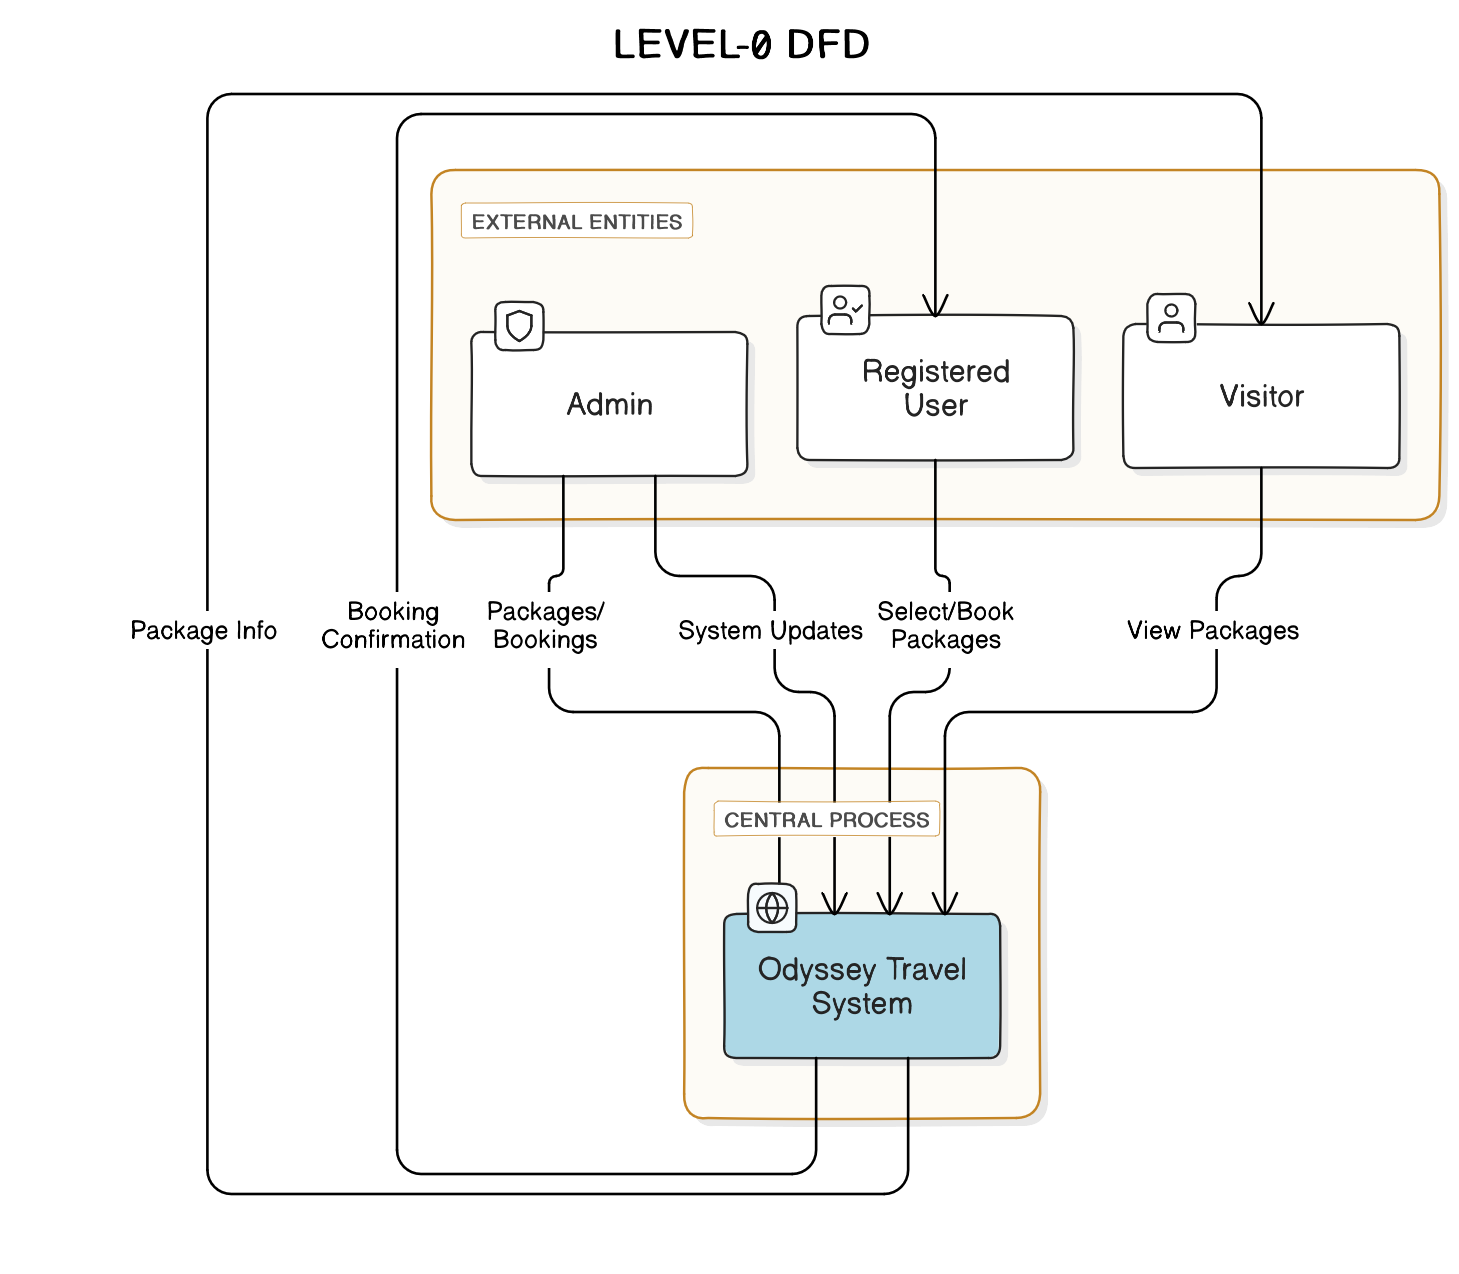
\includegraphics[width=500px, height=480px]{L0.png}}
\end{center}
\begin{center}

    \parbox{0.8\textwidth}{ 
        \centering
        \textbf{Figure - 3.1 : Level 0 Data Flow Diagram}
    }
\end{center}
\begin{center}
    {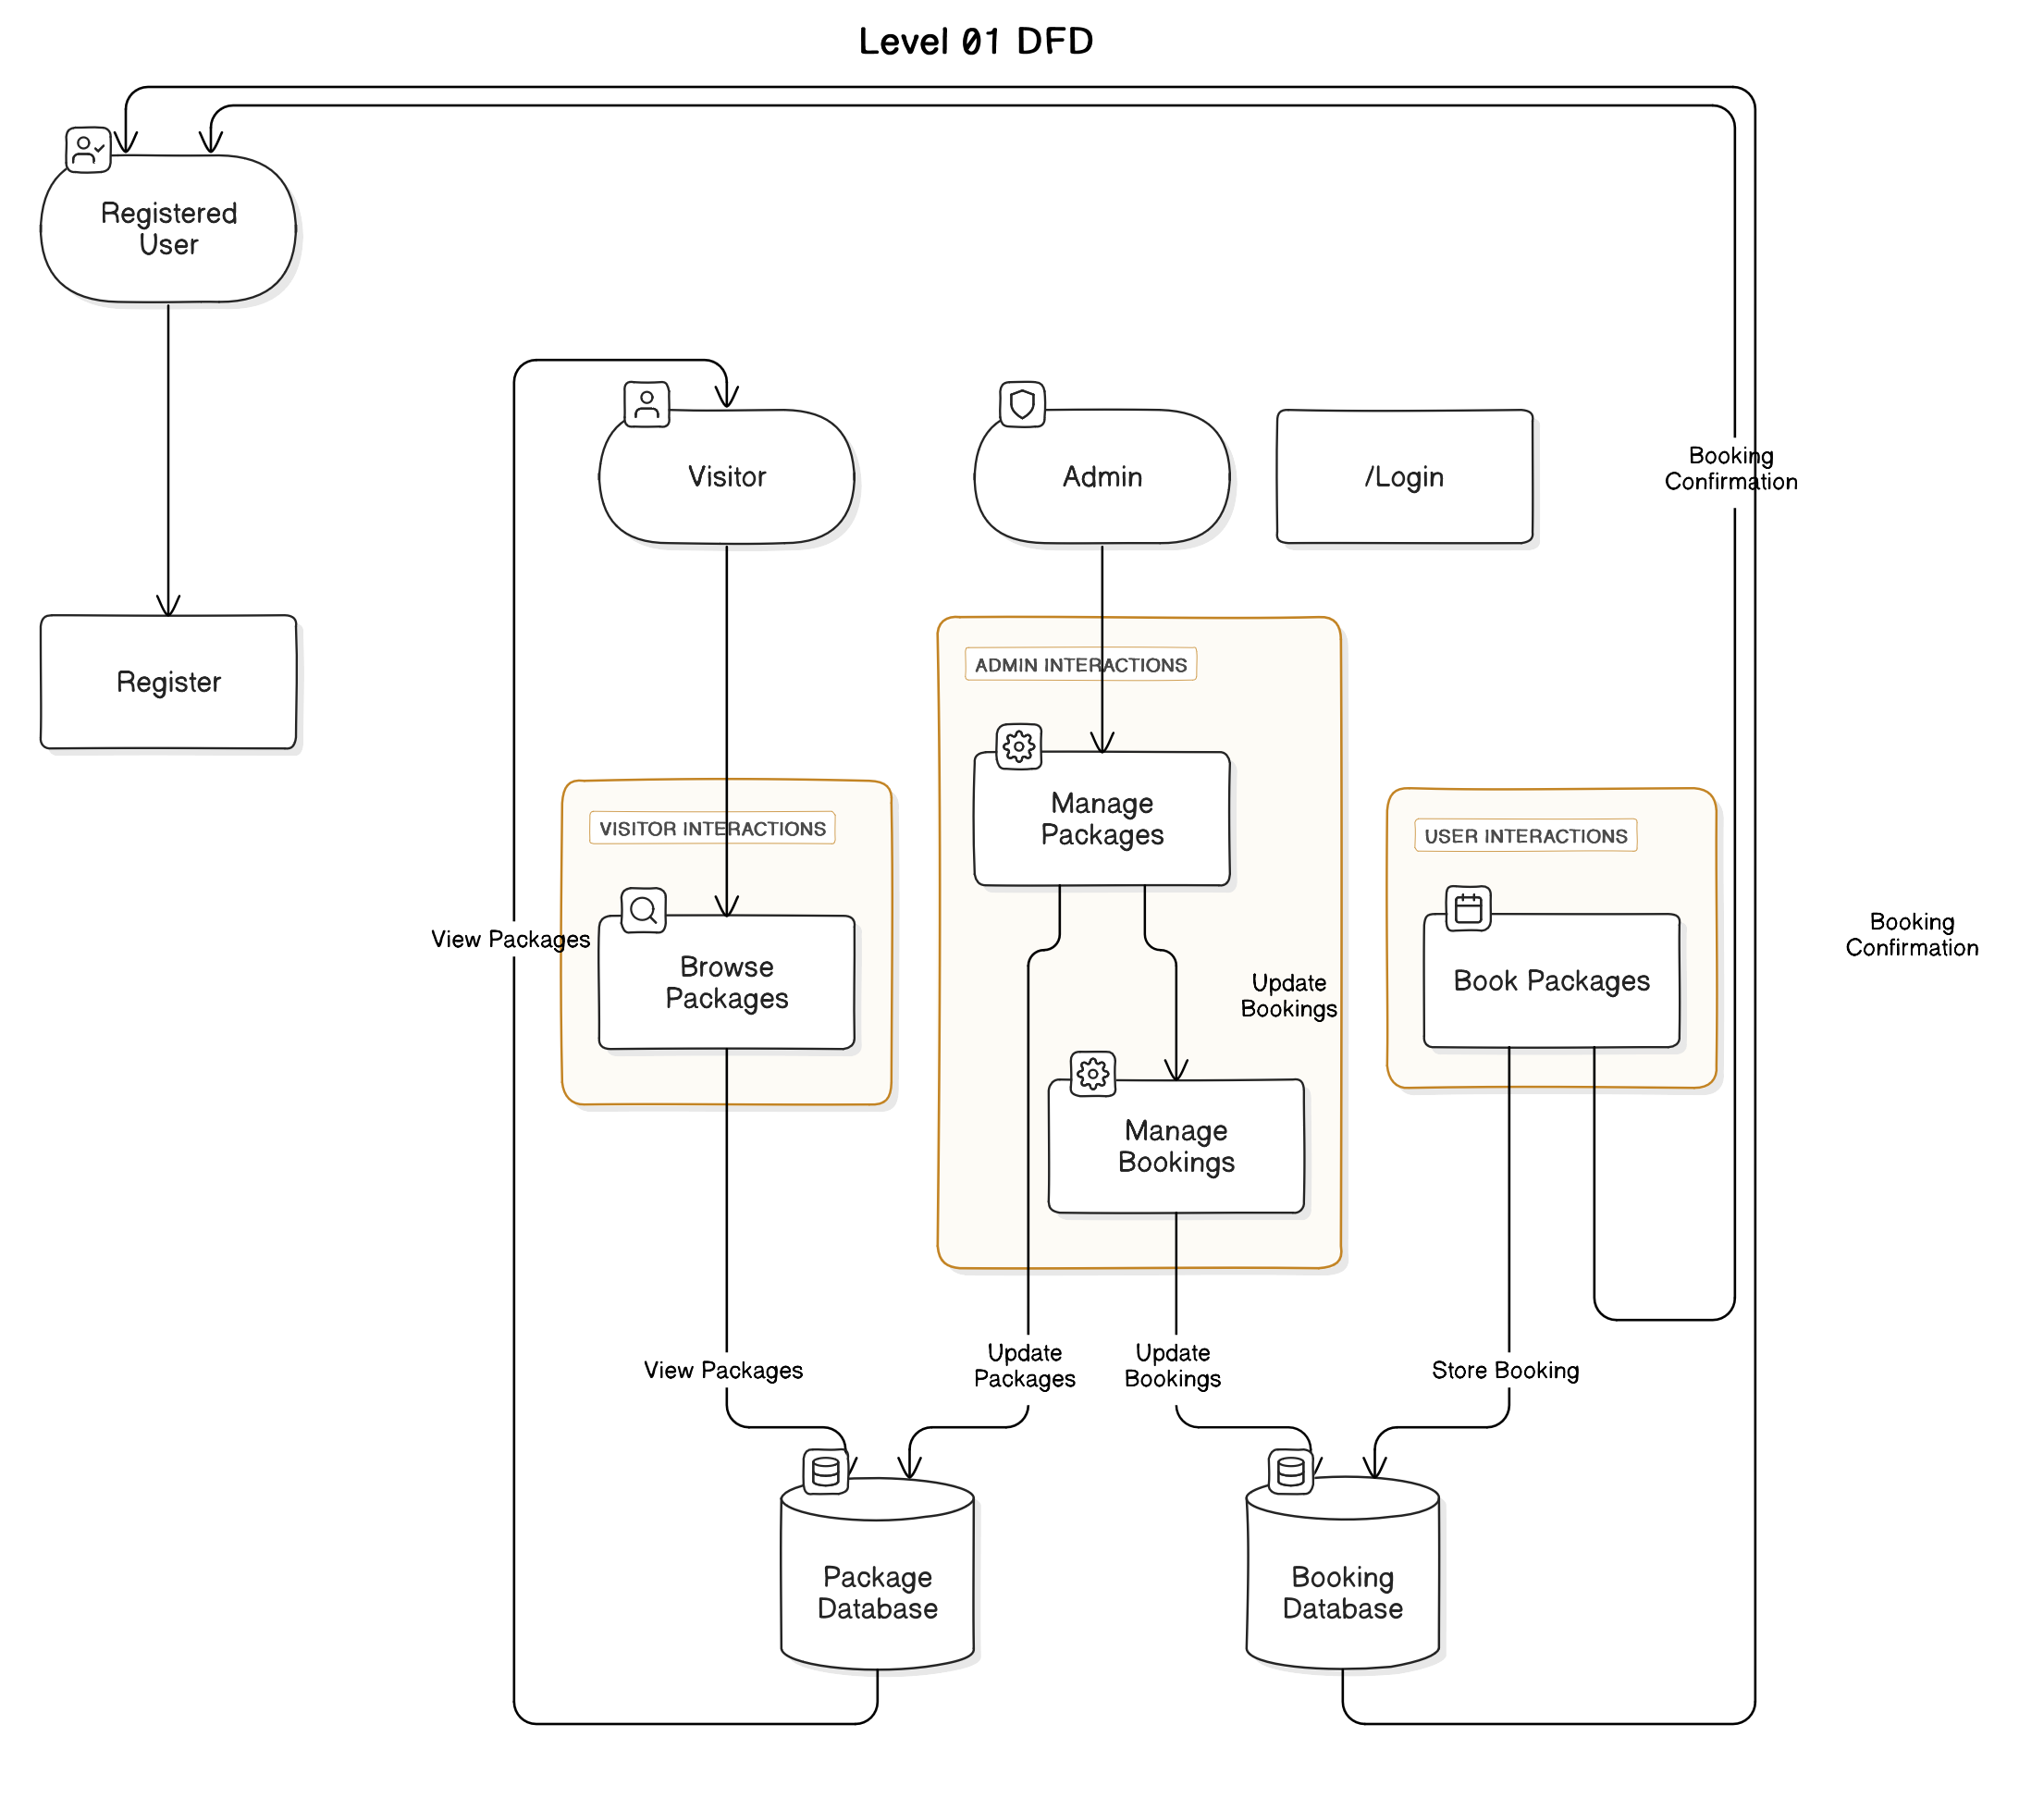
\includegraphics[width=500px, height=480px]{L1.png}}
\end{center}
\begin{center}

    \parbox{0.8\textwidth}{ 
        \centering
        \textbf{Figure - 3.1 : Level 1 Data Flow Diagram}
    }
\end{center}

\chapter{Test Case Design}

% Table 1 - TC001
\begin{longtable}{| m{2cm} | m{5cm} | m{4cm} | m{3cm} |}
\caption{Test Case for User Registration (TC001)}
\vspace{0.5cm} \\ \hline
\textbf{Test Case ID:} & \multicolumn{3}{l|}{TC001} \\ \hline
\textbf{Test Scenario:} & \multicolumn{3}{l|}{Verify successful user registration} \\ \hline
\textbf{Test Case:} & \multicolumn{3}{l|}{Register a new user on the platform} \\ \hline
\textbf{Pre-Condition:} & \multicolumn{3}{l|}{The user is on the registration page and has not registered before.} \\ \hline
\textbf{Test Steps} & \textbf{Test Data} & \textbf{Expected Result} & \textbf{Post Condition} \\ \hline
1. Navigate to the registration page. & URL: /register & The registration page loads successfully. & The user is presented with a registration form. \\ \hline
2. Enter a valid username. & Username: user123 & The username is accepted by the system. & The system accepts the username. \\ \hline
3. Enter a valid email. & Email: user@example.com & The email is accepted by the system. & The system accepts the email address. \\ \hline
4. Enter a secure password. & Password: Password123! & The password is accepted by the system. & The system accepts the password. \\ \hline
5. Click "Register". & N/A & The user is successfully registered and redirected to the login page with a confirmation message. & User account is created, and the system is updated with the new user details. \\ \hline
\end{longtable}

\vspace{1cm}
\newpage

% Table 2 - TC002
\begin{longtable}{| m{2cm} | m{5cm} | m{4cm} | m{3cm} |}
\caption{Test Case for User Login (TC002)}
\vspace{0.5cm} \\ \hline
\textbf{Test Case ID:} & \multicolumn{3}{l|}{TC002} \\ \hline
\textbf{Test Scenario:} & \multicolumn{3}{l|}{Verify successful user login} \\ \hline
\textbf{Test Case:} & \multicolumn{3}{l|}{Log in with valid credentials} \\ \hline
\textbf{Pre-Condition:} & \multicolumn{3}{l|}{The user must be registered and on the login page.} \\ \hline
\textbf{Test Steps} & \textbf{Test Data} & \textbf{Expected Result} & \textbf{Post Condition} \\ \hline
1. Navigate to the login page. & URL: /login & The login page loads successfully. & The user is presented with a login form. \\ \hline
2. Enter the registered email. & Email: user@example.com & The email is recognized by the system. & The system accepts the email address. \\ \hline
3. Enter the correct password. & Password: Password123! & The password is recognized by the system. & The system accepts the password. \\ \hline
4. Click "Login". & N/A & User successfully logs in and is redirected to the home page. & User session is initiated, and the user is logged into the system. \\ \hline
\end{longtable}

\vspace{1cm}

% Table 3 - TC003
\begin{longtable}{| m{2cm} | m{5cm} | m{4cm} | m{3cm} |}
\caption{Test Case for Viewing Travel Packages by Visitors (TC003)}
\vspace{0.5cm} \\ \hline
\textbf{Test Case ID:} & \multicolumn{3}{l|}{TC003} \\ \hline
\textbf{Test Scenario:} & \multicolumn{3}{l|}{Verify successful travel package viewing by visitors} \\ \hline
\textbf{Test Case:} & \multicolumn{3}{l|}{View travel packages as a visitor} \\ \hline
\textbf{Pre-Condition:} & \multicolumn{3}{l|}{User is not logged in and on the website's home page.} \\ \hline
\textbf{Test Steps} & \textbf{Test Data} & \textbf{Expected Result} & \textbf{Post Condition} \\ \hline
1. Navigate to the home page. & URL: /home & The home page loads successfully with the "Packages" menu option visible. & The visitor can see the available travel packages. \\ \hline
2. Click on the "Packages" menu option. & N/A & Visitor can view a list of available travel packages, including destination, duration, and price details. & System displays travel packages without requiring a user login. \\ \hline
\end{longtable}

\vspace{1cm}

% Table 4 - TC004
\begin{longtable}{| m{2cm} | m{5cm} | m{4cm} | m{3cm} |}
\caption{Test Case for Booking a Travel Package (TC004)}
\vspace{0.5cm} \\ \hline
\textbf{Test Case ID:} & \multicolumn{3}{l|}{TC004} \\ \hline
\textbf{Test Scenario:} & \multicolumn{3}{l|}{Verify successful booking of a travel package} \\ \hline
\textbf{Test Case:} & \multicolumn{3}{l|}{Book a travel package as a logged-in user} \\ \hline
\textbf{Pre-Condition:} & \multicolumn{3}{l|}{The user must be logged in and have access to the list of travel packages.} \\ \hline
\textbf{Test Steps} & \textbf{Test Data} & \textbf{Expected Result} & \textbf{Post Condition} \\ \hline
1. Log in to the platform. & Email: user@example.com \newline Password: Password123! & The user successfully logs in and accesses their account. & The user session is initiated. \\ \hline
2. Navigate to "Packages". & URL: /packages & The list of travel packages is displayed. & The user can view available travel packages. \\ \hline
3. Select a travel package. & Travel Package: Package1 & The selected package details are displayed, including booking options. & The user can proceed with the booking. \\ \hline
4. Click "Book Now". & N/A & The booking form is displayed with options to select dates and confirm the booking. & The user is ready to enter booking details. \\ \hline
5. Enter booking details. & Travel Dates: 2024-10-01 to 2024-10-07 & The booking details are accepted by the system. & The user is ready to confirm the booking. \\ \hline
6. Confirm the booking. & N/A & Booking is successfully processed, and the user receives a confirmation with booking details. & The booking is recorded in the system, and the booking confirmation is sent to the user. \\ \hline
\end{longtable}

\vspace{1cm}

% Table 5 - TC005
\begin{longtable}{| m{2cm} | m{5cm} | m{4cm} | m{3cm} |}
\caption{Test Case for Canceling a Travel Package Booking (TC005)}
\vspace{0.5cm} \\ \hline
\textbf{Test Case ID:} & \multicolumn{3}{l|}{TC005} \\ \hline
\textbf{Test Scenario:} & \multicolumn{3}{l|}{Verify successful cancellation of a booking} \\ \hline
\textbf{Test Case:} & \multicolumn{3}{l|}{Cancel a booked travel package} \\ \hline
\textbf{Pre-Condition:} & \multicolumn{3}{l|}{The user has an active booking and is logged in.} \\ \hline
\textbf{Test Steps} & \textbf{Test Data} & \textbf{Expected Result} & \textbf{Post Condition} \\ \hline
1. Log in to the platform. & Email: user@example.com \newline Password: Password123! & The user successfully logs in and accesses their account. & The user session is initiated. \\ \hline
2. Navigate to "My Bookings". & URL: /my-bookings & The user's active bookings are displayed. & The user can view their current bookings. \\ \hline
3. Select a booking. & Booking ID: BK12345 & The selected booking details are displayed with options to cancel the booking. & The user can proceed with cancellation. \\ \hline
4. Click "Cancel Booking". & N/A & The system prompts the user to confirm the cancellation. & The user can confirm or decline the cancellation request. \\ \hline
5. Confirm cancellation. & N/A & The booking is successfully canceled, and a confirmation is sent to the user. & The booking is removed from the user's active bookings, and the cancellation is recorded in the system. \\ \hline
\end{longtable}
% Table 6 - TC006
\begin{longtable}{| m{2cm} | m{5cm} | m{4cm} | m{3cm} |}
    \caption{Test Case for Adding a New Travel Package by Admin (TC006)}
    \vspace{0.5cm} \\ \hline
    \textbf{Test Case ID:} & \multicolumn{3}{l|}{TC006} \\ \hline
    \textbf{Test Scenario:} & \multicolumn{3}{l|}{Verify successful addition of a new travel package by admin} \\ \hline
    \textbf{Test Case:} & \multicolumn{3}{l|}{Admin adds a new travel package to the system} \\ \hline
    \textbf{Pre-Condition:} & \multicolumn{3}{l|}{Admin is logged into the system and has the required privileges.} \\ \hline
    \textbf{Test Steps} & \textbf{Test Data} & \textbf{Expected Result} & \textbf{Post Condition} \\ \hline
    1. Log in as admin. & Admin credentials & Admin successfully logs into the system. & Admin session is initiated. \\ \hline
    2. Navigate to the "Add Package" section. & URL: /admin/add-package & The "Add Package" form is displayed. & Admin can add a new package. \\ \hline
    3. Enter package details. & Package Name: Tropical Adventure \newline Price: \$2000 \newline Duration: 7 days & The package details are accepted by the system. & The system is ready to save the new package. \\ \hline
    4. Click "Save". & N/A & The package is successfully added and appears in the available travel packages list. & The new package is saved in the system. \\ \hline
    \end{longtable}
    
    \vspace{1cm}
    
    % Table 7 - TC007
    \begin{longtable}{| m{2cm} | m{5cm} | m{4cm} | m{3cm} |}
    \caption{Test Case for Modifying a Travel Package by Admin (TC007)}
    \vspace{0.5cm} \\ \hline
    \textbf{Test Case ID:} & \multicolumn{3}{l|}{TC007} \\ \hline
    \textbf{Test Scenario:} & \multicolumn{3}{l|}{Verify successful modification of an existing travel package by admin} \\ \hline
    \textbf{Test Case:} & \multicolumn{3}{l|}{Admin modifies a travel package details} \\ \hline
    \textbf{Pre-Condition:} & \multicolumn{3}{l|}{Admin is logged into the system and has the required privileges.} \\ \hline
    \textbf{Test Steps} & \textbf{Test Data} & \textbf{Expected Result} & \textbf{Post Condition} \\ \hline
    1. Log in as admin. & Admin credentials & Admin successfully logs into the system. & Admin session is initiated. \\ \hline
    2. Navigate to the "Packages" section. & URL: /admin/packages & The list of available packages is displayed. & Admin can select a package to modify. \\ \hline
    3. Select a package to modify. & Package Name: Tropical Adventure & The selected package details are displayed for modification. & Admin can make changes to the package. \\ \hline
    4. Update package details. & New Price: \$1800 & The updated package details are accepted by the system. & The system is ready to save the modified package. \\ \hline
    5. Click "Save". & N/A & The package is successfully updated in the system and reflects the modified details. & The changes are saved and reflected in the available travel packages. \\ \hline
    \end{longtable}
    
    \vspace{1cm}
    
    % Table 8 - TC008
    \begin{longtable}{| m{2cm} | m{5cm} | m{4cm} | m{3cm} |}
    \caption{Test Case for Deleting a Travel Package by Admin (TC008)}
    \vspace{0.5cm} \\ \hline
    \textbf{Test Case ID:} & \multicolumn{3}{l|}{TC008} \\ \hline
    \textbf{Test Scenario:} & \multicolumn{3}{l|}{Verify successful deletion of a travel package by admin} \\ \hline
    \textbf{Test Case:} & \multicolumn{3}{l|}{Admin deletes a travel package from the system} \\ \hline
    \textbf{Pre-Condition:} & \multicolumn{3}{l|}{Admin is logged into the system and has the required privileges.} \\ \hline
    \textbf{Test Steps} & \textbf{Test Data} & \textbf{Expected Result} & \textbf{Post Condition} \\ \hline
    1. Log in as admin. & Admin credentials & Admin successfully logs into the system. & Admin session is initiated. \\ \hline
    2. Navigate to the "Packages" section. & URL: /admin/packages & The list of available packages is displayed. & Admin can select a package to delete. \\ \hline
    3. Select a package to delete. & Package Name: Tropical Adventure & The system prompts the admin for confirmation before deleting the package. & Admin can proceed with deletion. \\ \hline
    4. Confirm deletion. & N/A & The package is successfully deleted from the system. & The package is removed from the list of available travel packages. \\ \hline
    \end{longtable}
    
    \vspace{1cm}
    
    % Table 9 - TC009
    \begin{longtable}{| m{2cm} | m{5cm} | m{4cm} | m{3cm} |}
    \caption{Test Case for Viewing Booking History by User (TC009)}
    \vspace{0.5cm} \\ \hline
    \textbf{Test Case ID:} & \multicolumn{3}{l|}{TC009} \\ \hline
    \textbf{Test Scenario:} & \multicolumn{3}{l|}{Verify successful viewing of booking history by the user} \\ \hline
    \textbf{Test Case:} & \multicolumn{3}{l|}{View booking history of a logged-in user} \\ \hline
    \textbf{Pre-Condition:} & \multicolumn{3}{l|}{User is logged in and has previous bookings.} \\ \hline
    \textbf{Test Steps} & \textbf{Test Data} & \textbf{Expected Result} & \textbf{Post Condition} \\ \hline
    1. Log in to the platform. & Email: user@example.com \newline Password: Password123! & User successfully logs in and accesses their account. & User session is initiated. \\ \hline
    2. Navigate to "My Bookings". & URL: /my-bookings & The user's booking history is displayed. & The user can view the list of past and current bookings. \\ \hline
    3. Select a booking. & Booking ID: BK12345 & The selected booking details are displayed, including travel dates and payment information. & User can view the complete booking details. \\ \hline
    \end{longtable}
    
    \vspace{1cm}
    
    % Table 10 - TC010
    \begin{longtable}{| m{2cm} | m{5cm} | m{4cm} | m{3cm} |}
    \caption{Test Case for Searching Travel Packages (TC010)}
    \vspace{0.5cm} \\ \hline
    \textbf{Test Case ID:} & \multicolumn{3}{l|}{TC010} \\ \hline
    \textbf{Test Scenario:} & \multicolumn{3}{l|}{Verify successful search of travel packages} \\ \hline
    \textbf{Test Case:} & \multicolumn{3}{l|}{Search for a travel package based on destination and price} \\ \hline
    \textbf{Pre-Condition:} & \multicolumn{3}{l|}{User is on the home page or package listing page.} \\ \hline
    \textbf{Test Steps} & \textbf{Test Data} & \textbf{Expected Result} & \textbf{Post Condition} \\ \hline
    1. Enter search criteria in the search bar. & Destination: Maldives \newline Price Range: \$1000-\$3000 & The system filters and displays packages matching the criteria. & User can view the filtered package list. \\ \hline
    2. Select a package from the search results. & Travel Package: Maldives Luxury & The selected package details are displayed. & User can proceed with the booking or view more details. \\ \hline
    \end{longtable}

    \chapter{Website Snapshots}

This chapter provides snapshots of the travel agency website, showcasing key functionalities such as viewing travel packages and user interface features.

\begin{figure}[h!]
    \centering
    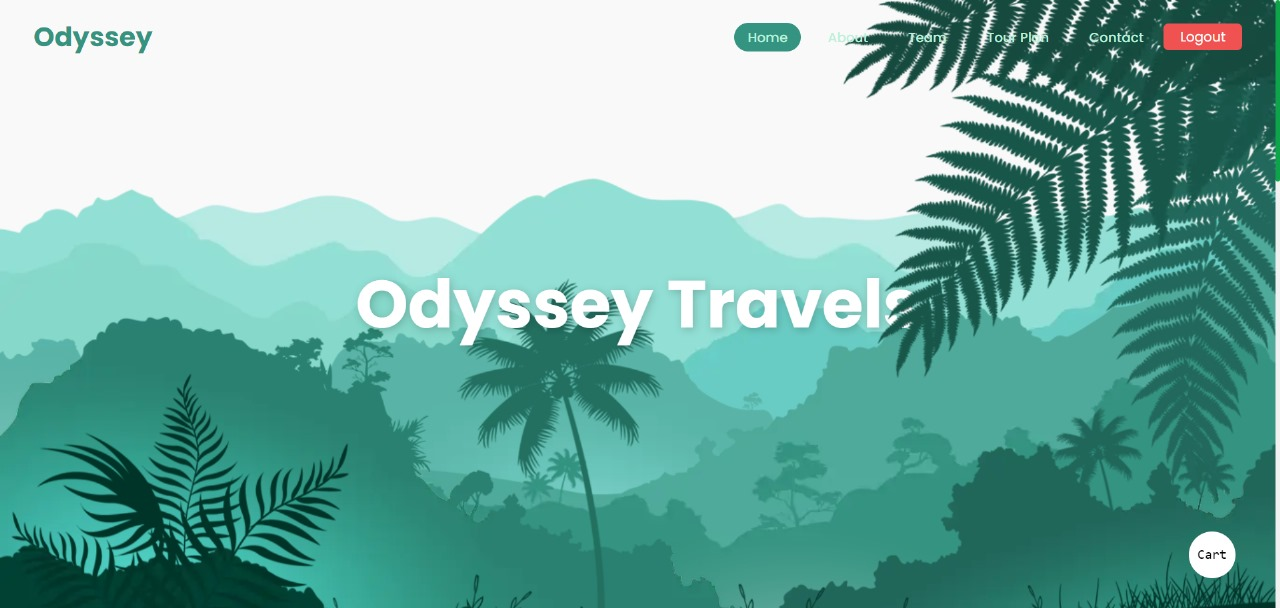
\includegraphics[width=1.1\textwidth, height=0.4\textheight]{./SS/home.jpg}
    \caption{Homepage displaying available travel packages}
    \label{fig:homepage}
\end{figure}

\begin{figure}[h!]
    \centering
    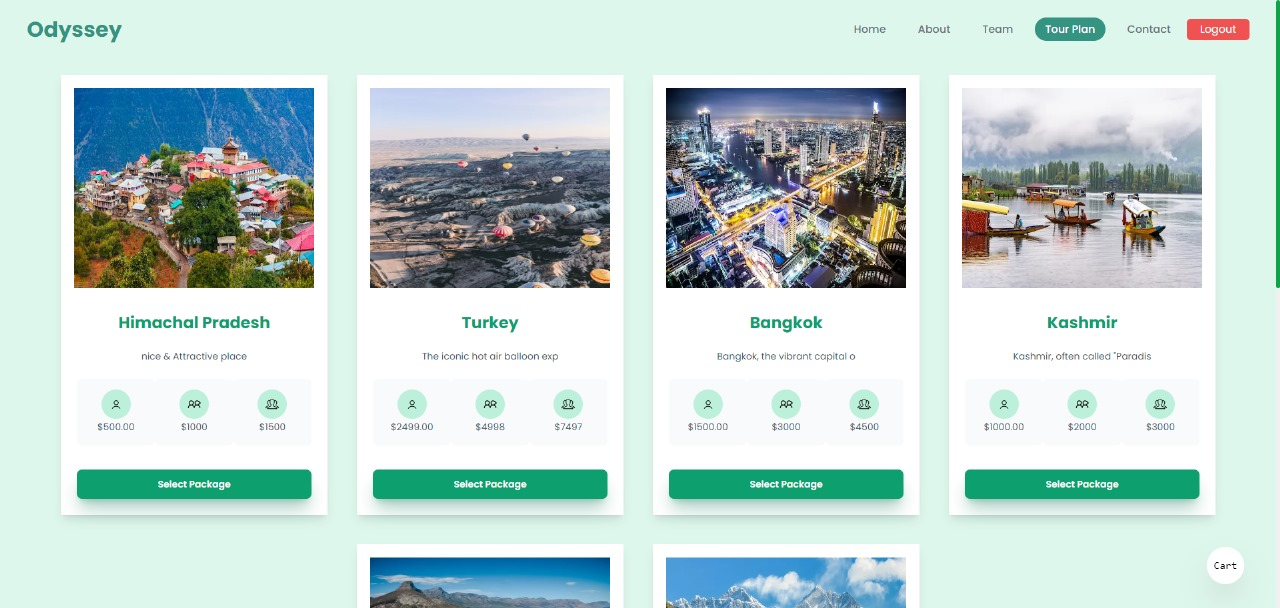
\includegraphics[width=1.1\textwidth, height=0.4\textheight]{./SS/plans.jpg}
    \caption{Travel plans overview page}
    \label{fig:plans}
\end{figure}

\begin{figure}[h!]
    \centering
    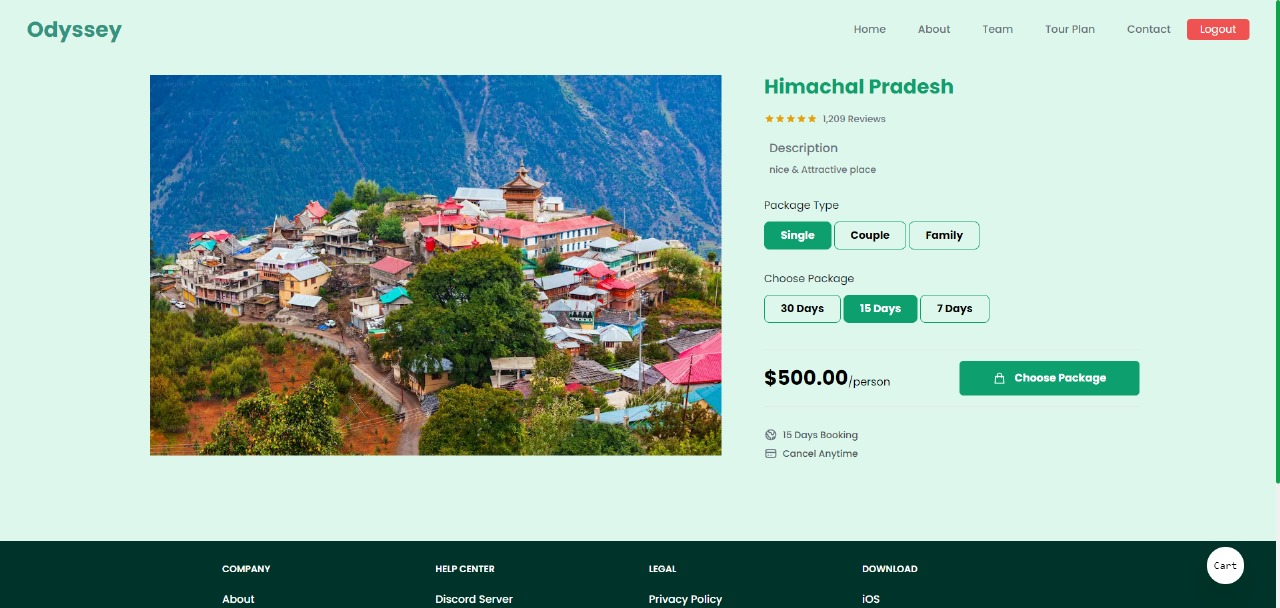
\includegraphics[width=1.1\textwidth, height=0.4\textheight]{./SS/plan.jpg}
    \caption{Detailed view of a selected travel plan}
    \label{fig:plan}
\end{figure}

\begin{figure}[h!]
    \centering
    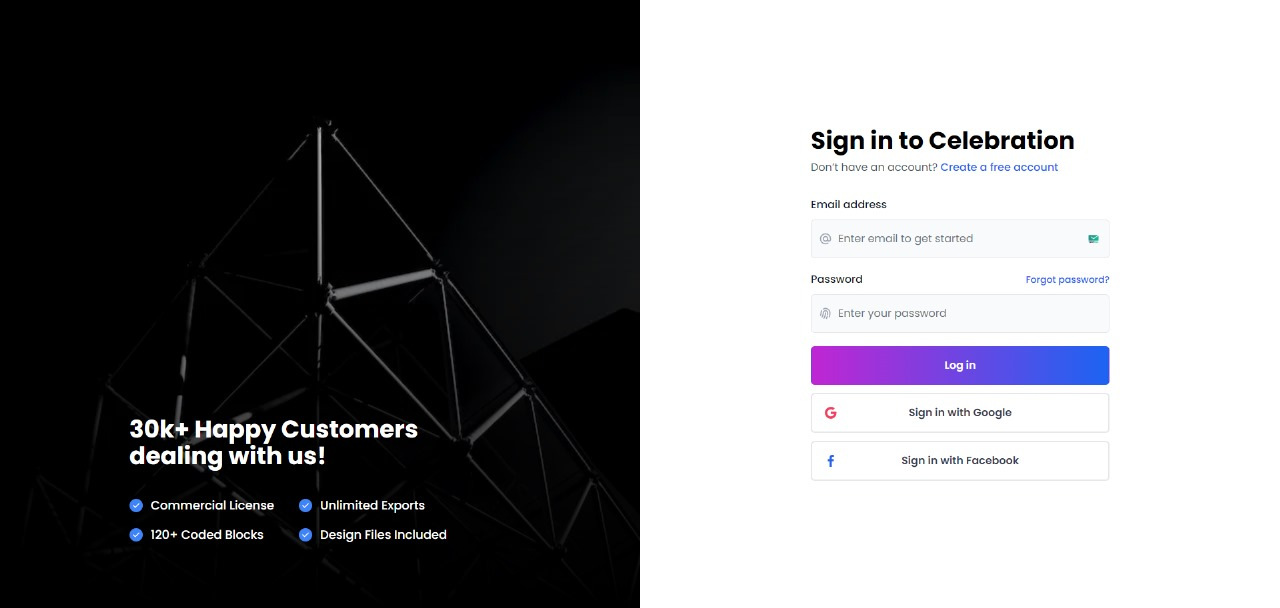
\includegraphics[width=1.1\textwidth, height=0.4\textheight]{./SS/signup.jpg}
    \caption{User sign-up page}
    \label{fig:signup}
\end{figure}

\begin{figure}[h!]
    \centering
    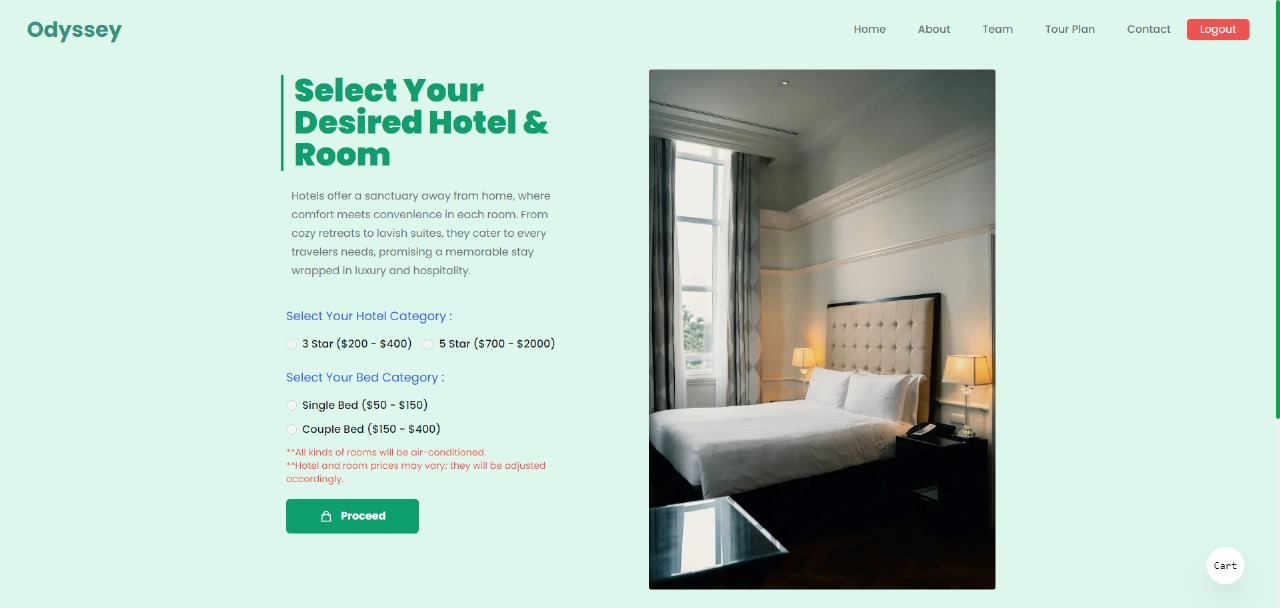
\includegraphics[width=1.1\textwidth, height=0.4\textheight]{./SS/hotel.jpg}
    \caption{Hotel booking interface}
    \label{fig:hotel}
\end{figure}

\begin{figure}[h!]
    \centering
    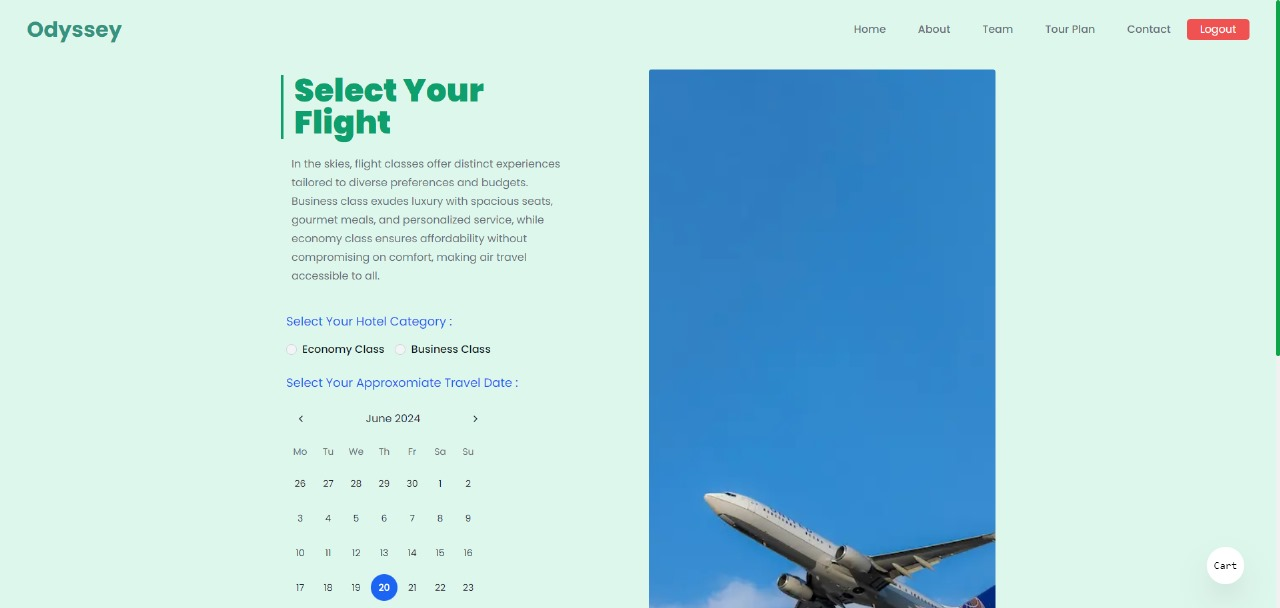
\includegraphics[width=1.1\textwidth, height=0.4\textheight]{./SS/flight.jpg}
    \caption{Flight booking interface}
    \label{fig:flight}
\end{figure}

\begin{figure}[h!]
    \centering
    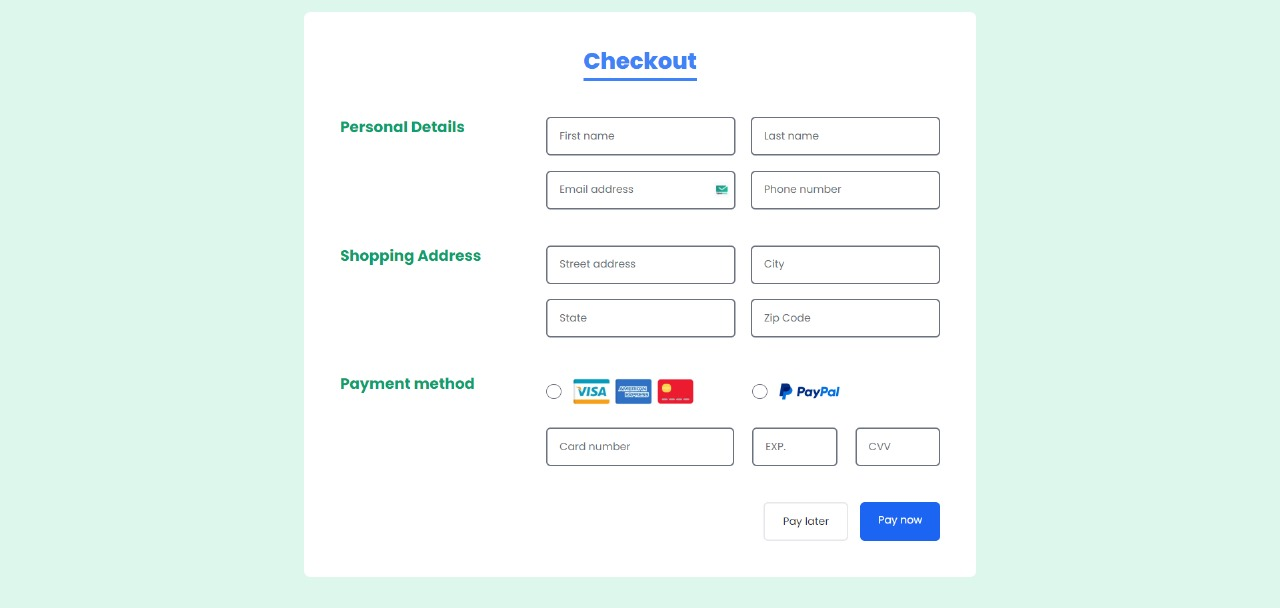
\includegraphics[width=1.1\textwidth, height=0.4\textheight]{./SS/payment.jpg}
    \caption{Payment gateway page}
    \label{fig:payment}
\end{figure}

\begin{figure}[h!]
    \centering
    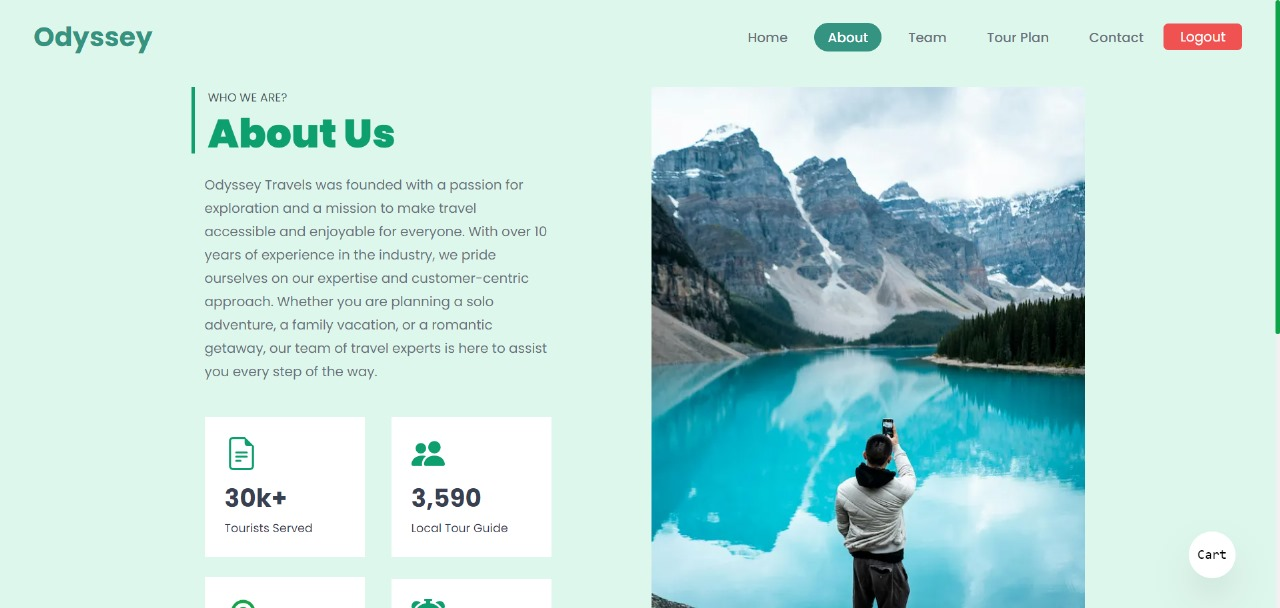
\includegraphics[width=1.1\textwidth, height=0.4\textheight]{./SS/about.jpg}
    \caption{About us page}
    \label{fig:about}
\end{figure}

\begin{figure}[h!]
    \centering
    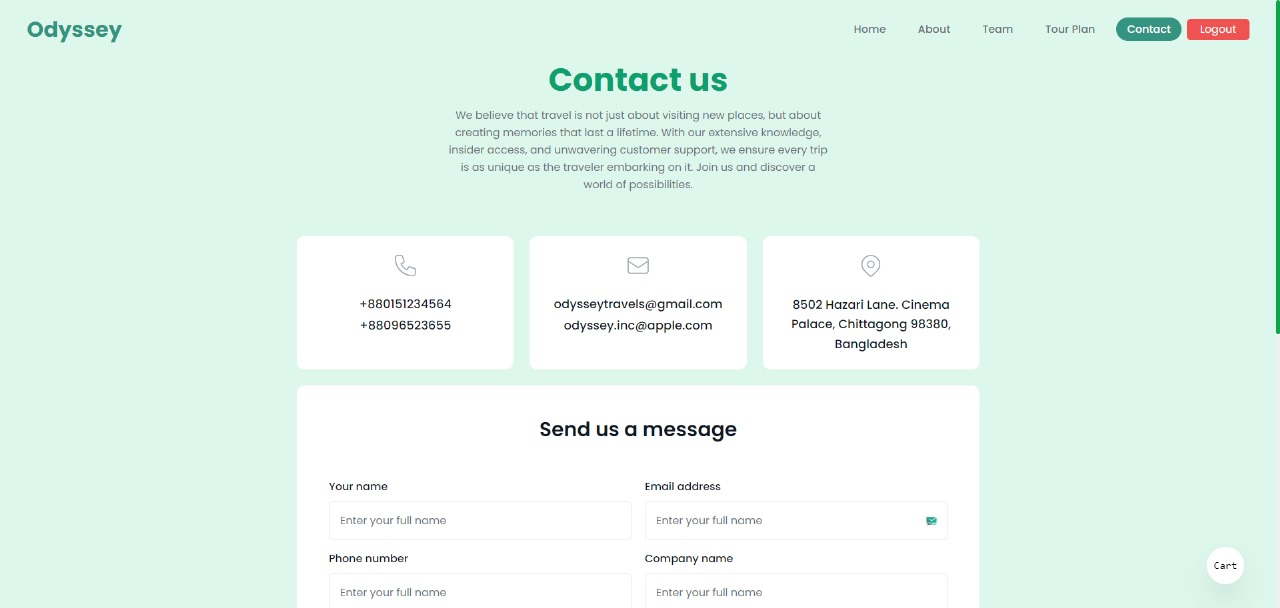
\includegraphics[width=1.1\textwidth, height=0.4\textheight]{./SS/contact_us.jpg}
    \caption{Contact us page}
    \label{fig:contact_us}
\end{figure}

\begin{figure}[h!]
    \centering
    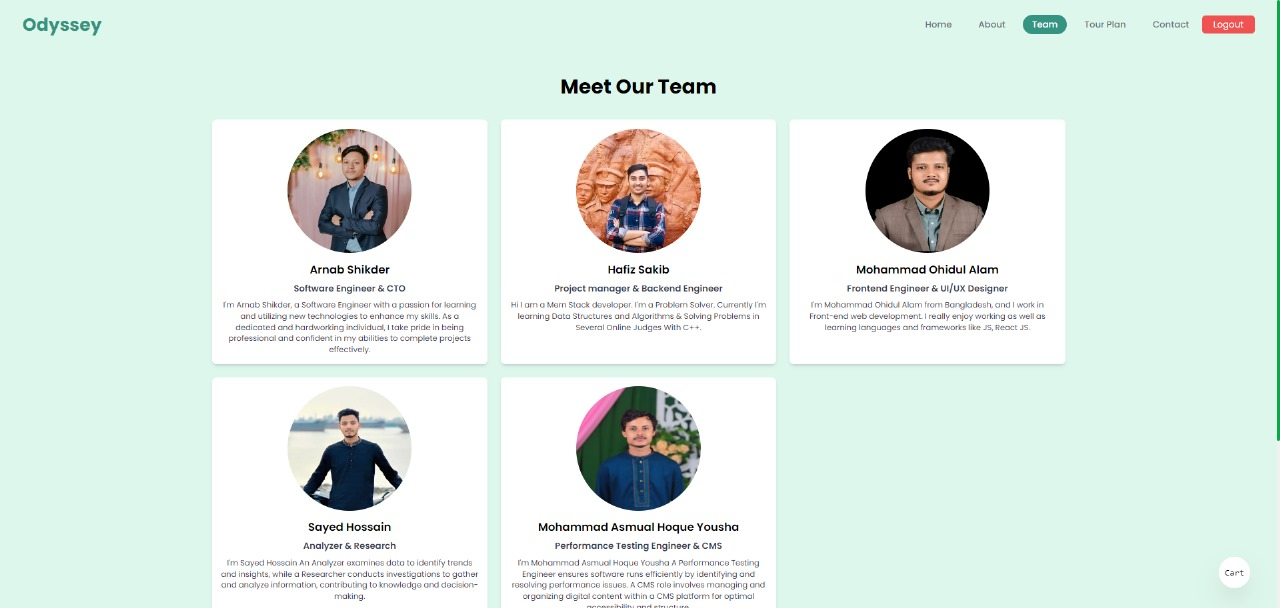
\includegraphics[width=1.1\textwidth, height=0.4\textheight]{./SS/developer.jpg}
    \caption{Developer page}
    \label{fig:developer}
\end{figure}

\begin{figure}[h!]
    \centering
    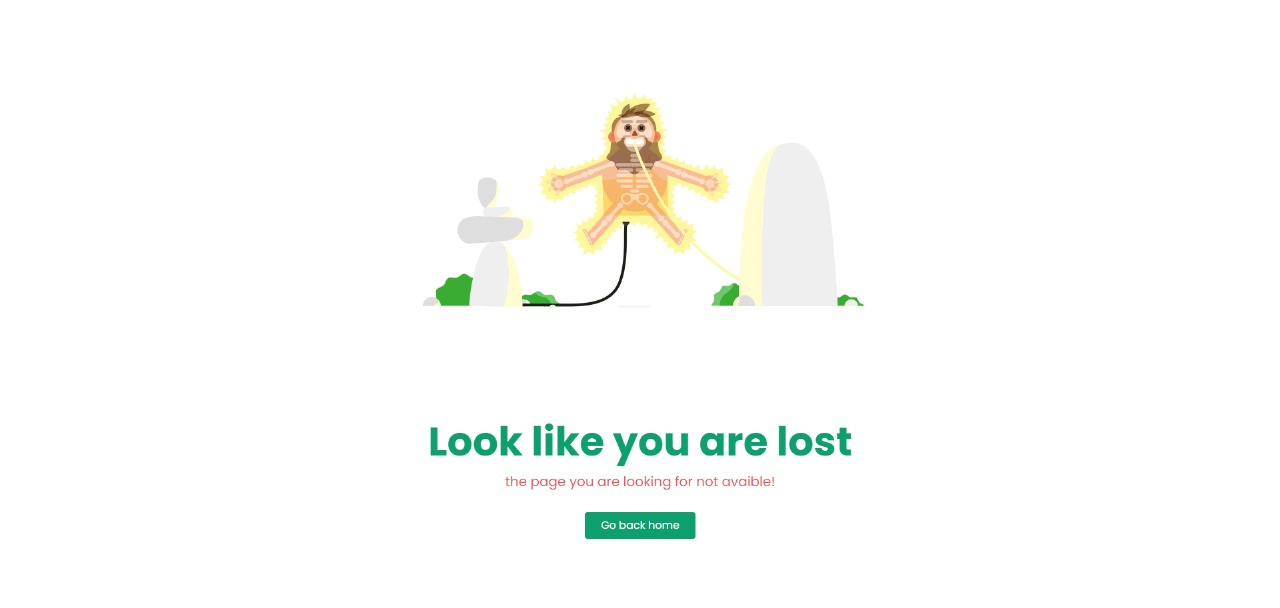
\includegraphics[width=1.1\textwidth, height=0.4\textheight]{./SS/error.jpg}
    \caption{Error page (404 not found)}
    \label{fig:error}
\end{figure}

\begin{figure}[h!]
    \centering
    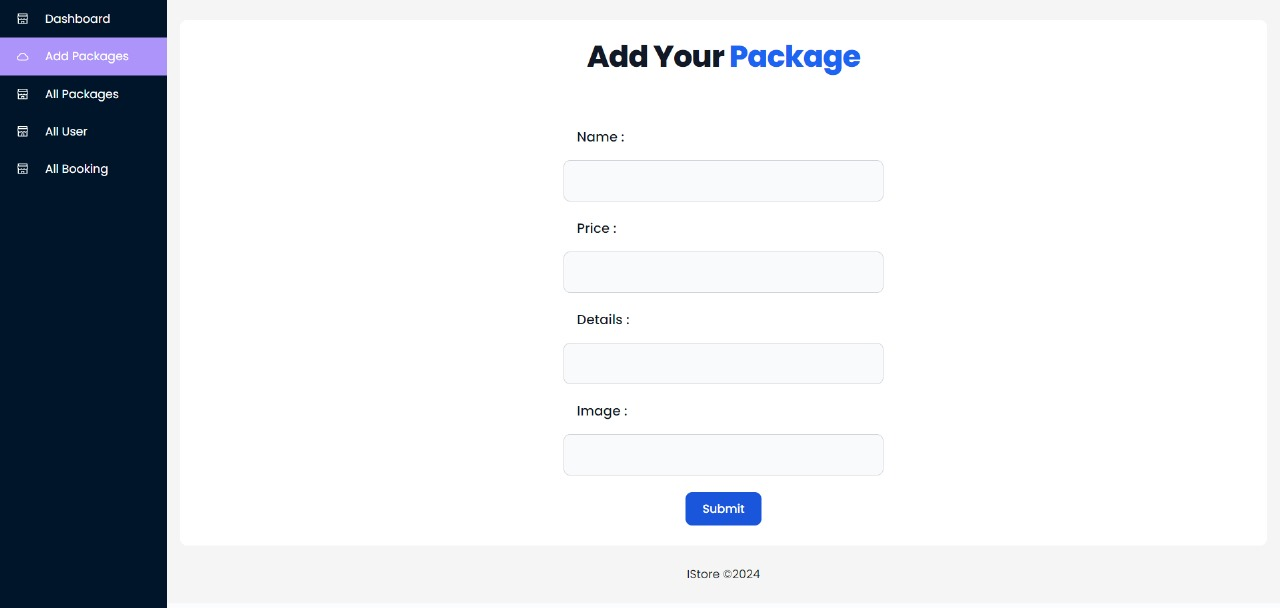
\includegraphics[width=1.1\textwidth, height=0.4\textheight]{./SS/admin.jpg}
    \caption{Admin dashboard}
    \label{fig:admin}
\end{figure}

\begin{figure}[h!]
    \centering
    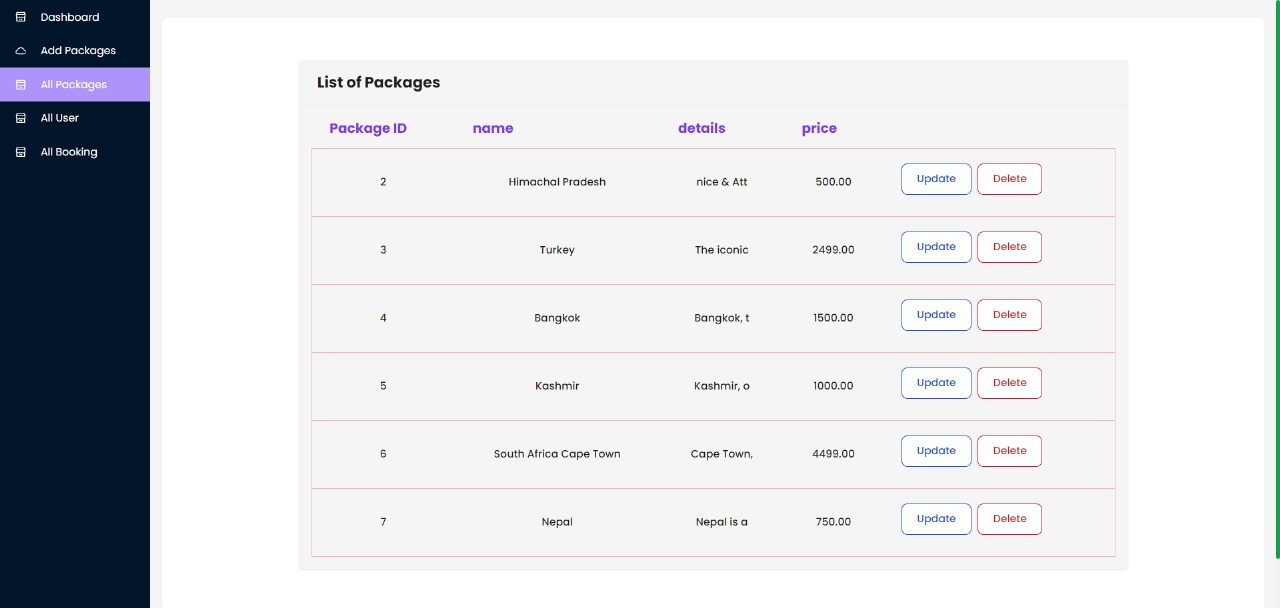
\includegraphics[width=1.1\textwidth, height=0.4\textheight]{./SS/manage_plan.jpg}
    \caption{Admin interface to manage travel plans}
    \label{fig:manage_plan}
\end{figure}

\begin{figure}[h!]
    \centering
    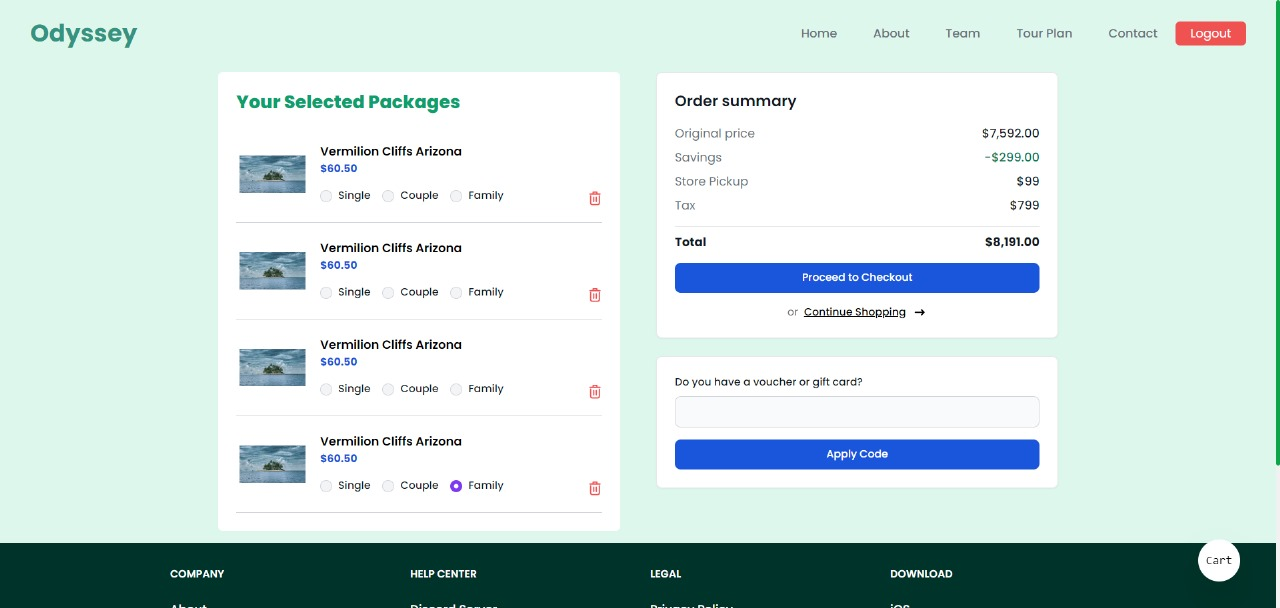
\includegraphics[width=1.1\textwidth, height=0.4\textheight]{./SS/pkg_edit.jpg}
    \caption{Admin interface to edit travel packages}
    \label{fig:pkg_edit}
\end{figure}

\chapter{Future Work}
In the future, the travel agency software can be improved with several key features to enhance user experience and system functionality. Below are some potential areas for future work:

\begin{itemize}
    \item \textbf{Recommendation System:} Implement a machine learning-based recommendation engine that suggests travel packages, accommodations, and transportation options based on user preferences and past behavior, improving customer satisfaction through personalized suggestions.
    
    \item \textbf{Real-time Data Integration:} Integrate third-party APIs to provide real-time data on flight and hotel availability, allowing users to make seamless bookings without delays in information.
    
    \item \textbf{Review and Rating System:} Develop a user review and rating system where users can share their experiences and feedback, helping future customers make informed decisions based on peer reviews.
    
    \item \textbf{Security Enhancements:} Strengthen the security of the platform by implementing advanced encryption methods, two-factor authentication, and improved data privacy protocols to safeguard user information and transaction data.
    
    \item \textbf{Multi-language and Currency Support:} Expand the platform to support multiple languages and currencies, making it accessible and user-friendly for a global audience.
    
    \item \textbf{Mobile Application Development:} Create a mobile application that mirrors the website’s functionality, allowing users to manage bookings, view travel details, and receive notifications on the go, offering greater convenience.
\end{itemize}

\chapter{Conclusion}

In conclusion, the development of the travel agency website successfully addresses the primary goal of providing both visitors and logged-in users with a seamless experience for browsing and selecting travel packages, transportation, and hotel bookings. The platform is designed with an intuitive user interface, making it accessible for all types of users, whether they are simply browsing or actively booking services.

Through the use of modern technologies such as Node.js, Next.js, MySQL, and Tailwind CSS, the system is highly responsive and efficient, ensuring smooth operation and performance. Additionally, the integration of user authentication allows for a personalized experience, with logged-in users gaining access to additional features such as customized package selection and bookings.

This project not only fulfills the requirements of our academic coursework but also serves as a practical solution that can be implemented in a real-world scenario. Moving forward, future enhancements could focus on expanding features like real-time booking confirmations, advanced search functionalities, and integration with third-party services for travel insurance or payment gateways.

Overall, this project demonstrates a successful blend of technical skill, project management, and a deep understanding of the end-user's needs, ensuring a valuable and functional product for a travel agency.


\end{document}